
\section{Krigsløb}

\subsubsection*{\textbf{Ansvarlige:} \Randildo \& \Stive}
\textbf{Tid:} 10:00 - 12:00. \\
Vektorer sætter poster op fra 9.35-9.50 \\
Russerne samles 9.50 \\
Løbet foregår i tværhold.

\subsection{Rotationsskema \Hashtag{LigesomUnderSex}}
\begin{table}[H]
\centering
\begin{tabu}{l *{8}{C{1.4cm}}}\specialrule{1pt}{0pt}{2pt}
\rowfont{\bfseries}
Tid   & Post 1   & Post 2   & Post 3   & Post 4   & Post 5   & Post 6   & Post 7   & Post 8   \\ \specialrule{1pt}{2pt}{2pt}
10:00 & Austral  & Skotland & Indien   & Viking   & Egypten  & 'Murica  & Brasil   & Ølymp    \\ \specialrule{.25pt}{1pt}{1pt}
10:15 & Ølymp    & Austral  & Skotland & Indien   & Viking   & Egypten  & 'Murica  & Brasil   \\ \specialrule{.25pt}{1pt}{1pt}
10:30 & Brasil   & Ølymp    & Austral  & Skotland & Indien   & Viking   & Egypten  & 'Murica  \\ \specialrule{.25pt}{1pt}{1pt}
10:45 & 'Murica	 & Brasil   & Ølymp    & Austral  & Skotland & Indien   & Viking   & Egypten  \\ \specialrule{.25pt}{1pt}{1pt}
11:00 & Egypten  & 'Murica  & Brasil   & Ølymp    & Austral  & Skotland & Indien   & Viking   \\ \specialrule{.25pt}{1pt}{1pt}
11:15 & Viking   & Egypten  & 'Murica  & Brasil   & Ølymp    & Austral  & Skotland & Indien   \\ \specialrule{.25pt}{1pt}{1pt}
11:30 & Indien	 & Viking   & Egypten  & 'Murica  & Brasil   & Ølymp    & Austral  & Skotland \\ \specialrule{.25pt}{1pt}{1pt}
11:45 & Skotland & Indien   & Viking   & Egypten  & 'Murica  & Brasil   & Ølymp    & Austral  \\ \specialrule{1pt}{2pt}{0pt}
\end{tabu}
\end{table}

\subsection{Posterne}

\subsubsection*{Oversigt}
\begin{enumerate}
  \item Krokodilleleg - \Stive - Foran shelterne
  \item Kampråb - \Mighty - Store græsplæne
  \item Klodsmajor - \Buddha - Pejsestuen
  \item Vikingekast - \Karla - Lille græsplæne
  \item Mumificering - \Farav - Græsplæne foran køkkenet
  \item Skyd efter dåser - \Clint - Spisesalen
  \item Skyd igennem hulahopringe - \Randildo - Store græsplæne
  \item Gurgle yogurt - \Hemorides - Gården
\end{enumerate}

\begin{figure}[H]
\centering
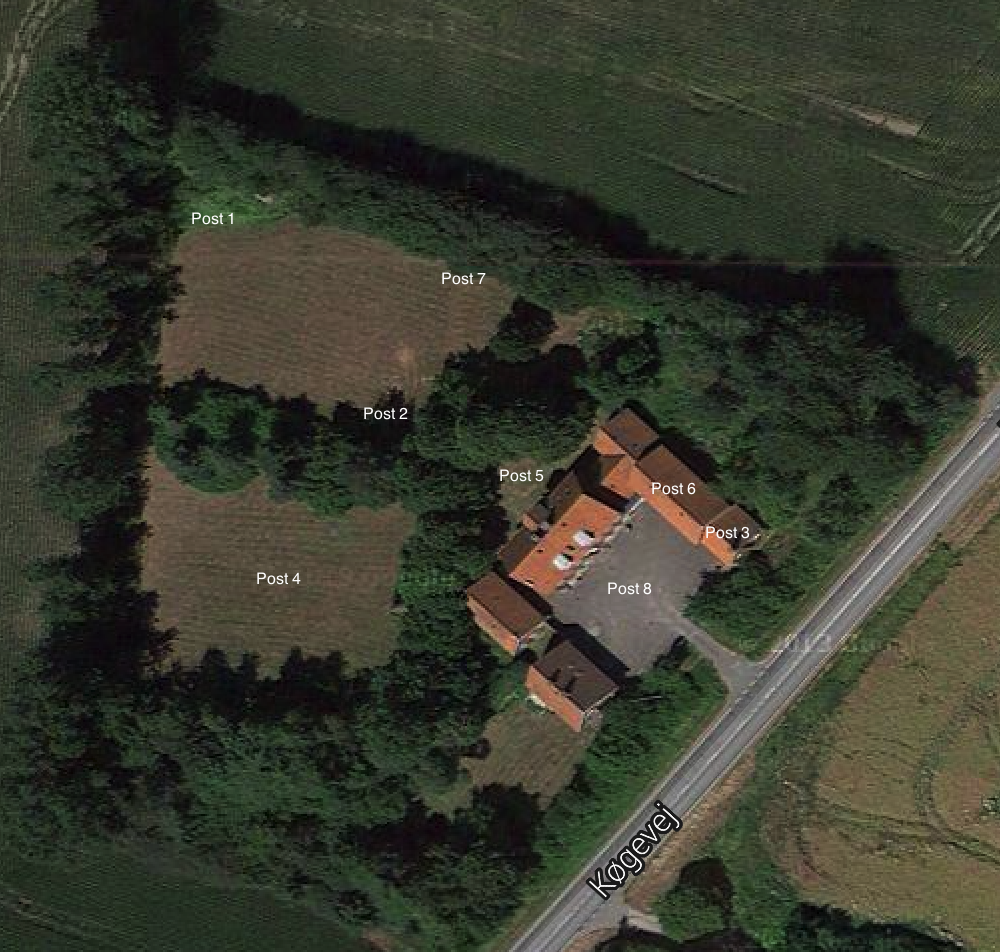
\includegraphics[width=\linewidth]{fig/KrigsPoster.png}
\end{figure}

\pagebreak

%%%%%%%%%%%%%%%%%%% Post 1 %%%%%%%%%%%%%%%%%%%
\subsubsection*{\textbf{Post 1 –  Krokodilleleg}}
\subsubsection*{\textbf{Ansvarlig: \Stive}} 
\textbf{Sted:} Foran shelterne \\
\textbf{Tid:} 15 minutter(inklusiv gang) \\
\textbf{Materialer:}
\begin{itemize}
  \item 2 ruller snor
  \item 1 lagen
  \item 4 ølkasser
  \item Saks
  \item Kuglepen
  \item Stopur
\end{itemize}
\textbf{Beskrivelse:} Legen kører i 8 minutter. Der sættes et stopur. 
Holdet deles lige op, den ene del er fangerholdet og de andre er krokodiller. Fangerholdet binder deres ben sammen, så alle har hvert ben bundet til to andre fra holdet (de danner én lang kæde). Krokodillen får begge ben bundet stramt sammen. Krokodillerne placeres rundt på græsplænen og fangerholdet skal nu transportere krokodillerne til et bestemt sted, uden at krokodillerne rører jorden (De skal bæres i lagnet). Spillet stoppes når alle tre er fanget. Der gives point fra 1 til 10 for bestikkelse, udførsel og tid. \\ 
\begin{table}[H]
\caption{\underline{Point på Krokodilleleg}}
\centering
\begin{tabu}{L{3.5cm} *{4}{|C{2.5cm}}}\specialrule{1pt}{0pt}{2pt}
\rowfont{\bfseries}
Hold & Tid & Udførsel & Bestikkelse & Samlet \\ \specialrule{1pt}{2pt}{2pt}
Brasilien       & & & & \\ \specialrule{.25pt}{1pt}{1pt}
Ølympen         & & & & \\ \specialrule{.25pt}{1pt}{1pt}
Skotland        & & & & \\ \specialrule{.25pt}{1pt}{1pt}
Sydøstasien     & & & & \\ \specialrule{.25pt}{1pt}{1pt}
Vikingeland     & & & & \\ \specialrule{.25pt}{1pt}{1pt}
'Murica!        & & & & \\ \specialrule{.25pt}{1pt}{1pt}
Australien      & & & & \\ \specialrule{.25pt}{1pt}{1pt}
Ægypten         & & & & \\ \specialrule{1pt}{2pt}{0pt}
\end{tabu}
\end{table}
\textbf{Næste post:} Post 2 - Kampråb - \Mighty

\pagebreak

%%%%%%%%%%%%%%%%%%% Post 2 %%%%%%%%%%%%%%%%%%%
\subsubsection*{\textbf{Post 2 - Kampråb}}
\subsubsection*{\textbf{Ansvarlig:} \Mighty}
\textbf{Sted:} Store græsplæne \\
\textbf{Tid:} 15 minutter (inklusiv gang) \\
\textbf{Materialer:}
\begin{itemize}
  \item Kuglepen
  \item Stopur
\end{itemize}
\textbf{Beskrivelse:} 
Legen kører i 8 minutter. Der sættes et stopur. Bedste kampråb. Der gives point fra 1 til 10 for awesomeness, kreativitet og bestikkelse. Mighty bonder med russerne hvis, der er mere tid til overs. \\
\begin{table}[H]
\caption{\underline{Point på Kampråb}}
\centering
\begin{tabu}{L{3.5cm} *{4}{|C{2.5cm}}}\specialrule{1pt}{0pt}{2pt}
\rowfont{\bfseries}
Hold & Awesomeness & Kreativitet & Bestikkelse & Samlet \\ \specialrule{1pt}{2pt}{2pt}
Brasilien       & & & & \\ \specialrule{.25pt}{1pt}{1pt}
Ølympen         & & & & \\ \specialrule{.25pt}{1pt}{1pt}
Skotland        & & & & \\ \specialrule{.25pt}{1pt}{1pt}
Sydøstasien     & & & & \\ \specialrule{.25pt}{1pt}{1pt}
Vikingeland     & & & & \\ \specialrule{.25pt}{1pt}{1pt}
'Murica!        & & & & \\ \specialrule{.25pt}{1pt}{1pt}
Australien      & & & & \\ \specialrule{.25pt}{1pt}{1pt}
Ægypten         & & & & \\ \specialrule{1pt}{2pt}{0pt}
\end{tabu}
\end{table}
\textbf{Næste post:} Post 3 - Klodsmajor - \Buddha

\pagebreak

%%%%%%%%%%%%%%%%%%% Post 3 %%%%%%%%%%%%%%%%%%%
\subsubsection*{\textbf{Post 3 – Klodsmajor}}
\subsubsection*{\textbf{Ansvarlig:} \Buddha}
\textbf{Sted:} Pejsestuen \\
\textbf{Tid:} 15 minutter (inklusiv gang) \\ 
\textbf{Materialer:}
\begin{itemize}
  \item Klodsmajor
  \item Stopur
\end{itemize}
\textbf{Beskrivelse:} Legen kører i 8 minutter. Der sættes et stopur. Buddha opsætter et spil klodsmajor inden hvert hold kommer. Hver person på holdet skal på skift fjerne en klods fra tårnet (aldrig den øverste) og klodsen lægges ovenpå tårnet. Der tælles hvor mange klodser, der tages ud, og det noteres. Hvis tårnet vælter, nulstilles antal klodser fra tidligere forsøg og holdet prøver igen. Antal klodser fjernet noteres. Der gives point fra 1 til 10 for bestikkelse og koncentration. \\
\begin{table}[H]
\caption{\underline{Point på Klodmajor på tid}}
\centering
\begin{tabu}{L{3.5cm} *{3}{|C{2.5cm}}}
\specialrule{1pt}{0pt}{2pt}
\rowfont{\bfseries}
Hold & Antal klodser & Bestikkelse & Samlet \\ \specialrule{1pt}{2pt}{2pt}
Brasilien       & & & \\ \specialrule{.25pt}{1pt}{1pt}
Ølympen         & & & \\ \specialrule{.25pt}{1pt}{1pt}
Skotland        & & & \\ \specialrule{.25pt}{1pt}{1pt}
Sydøstasien     & & & \\ \specialrule{.25pt}{1pt}{1pt}
Vikingeland     & & & \\ \specialrule{.25pt}{1pt}{1pt}
'Murica!        & & & \\ \specialrule{.25pt}{1pt}{1pt}
Australien      & & & \\ \specialrule{.25pt}{1pt}{1pt}
Ægypten         & & & \\ 
\specialrule{1pt}{2pt}{0pt}
\end{tabu}
\end{table}
\textbf{Næste post:} Post 4 - Vikingekast - \Karla

\pagebreak

%%%%%%%%%%%%%%%%%%% Post 4 %%%%%%%%%%%%%%%%%%%
\subsubsection*{\textbf{Post 4 – Spydkast}} 
\subsubsection*{\textbf{Ansvarlig:} \Karla (\Mighty som backup)}
\textbf{Sted:} Lille græsplæne \\
\textbf{Tid:} 15 minutter (inklusiv gang) \\
\textbf{Materialer:}
\begin{itemize}
\item Klodser fra Kongespil (tag alle fra spillet)
\item Målebånd (3/5 m fra værkstøjskasse)
\item Papir (til at notere længste/korteste kast)
\item Kuglepen
\item Skilte med meter (-3, 3, 6, 9, 12, 15, 18, ? m)
\item Stopur
\end{itemize}
\textbf{Beskrivelse:} Legen kører i 8 minutter eller til alle er færdige (ikke mere end 10 minutter). Der sættes et stopur. Der sættes skilte ud, som måles op inden løbet starter. Der skal kastes 30 gange i alt, det længste og korteste kast noteres. Der skal råbes som ægte vikinger inden, der kastes. Der gives point fra 1 til 10 for bestikkelse. Kast: Baglæns mellem benene, baglæns over hovedet, spasser hånds (underhåndskast), under en rus (point for kreativitet), baglæns over hovedet. \\
\begin{table}[H]
\caption{\underline{Point på Spydkast}}
\centering
\begin{tabu}{L{3.5cm} *{3}{|C{2.5cm}}}
\specialrule{1pt}{0pt}{2pt}
\rowfont{\bfseries}
Hold & Længde & Bestikkelse & Samlet \\ \specialrule{1pt}{2pt}{2pt}
Brasilien       & & & \\ \specialrule{.25pt}{1pt}{1pt}
Ølympen         & & & \\ \specialrule{.25pt}{1pt}{1pt}
Skotland        & & & \\ \specialrule{.25pt}{1pt}{1pt}
Sydøstasien     & & & \\ \specialrule{.25pt}{1pt}{1pt}
Vikingeland     & & & \\ \specialrule{.25pt}{1pt}{1pt}
'Murica!        & & & \\ \specialrule{.25pt}{1pt}{1pt}
Australien      & & & \\ \specialrule{.25pt}{1pt}{1pt}
Ægypten         & & & \\ 
\specialrule{1pt}{2pt}{0pt}
\end{tabu}
\end{table}
\textbf{Næste post:} Post 5 - Mumificering - \Farav

\pagebreak

%%%%%%%%%%%%%%%%%%% Post 5 %%%%%%%%%%%%%%%%%%%
\subsubsection*{\textbf{Post 5 – Mumificering}} 
\subsubsection*{\textbf{Ansvarlig:} \Farav}
\textbf{Sted:} Græsplæne foran køkkenet \\
\textbf{Tid:} 15 minutter (inklusiv gang) \\ 
\textbf{Materialer:}
\begin{itemize}
   \item Vitawrap
   \item Saks
   \item Stopur
\end{itemize}
\textbf{Beskrivelse:} Der bruges ca. 8 minutter på legen. Hvert hold skal pakke 3 personer ind individuelt i vitawrap hurtigst muligt. Der tages tid fra man starter med at pakke første person ind til den sidste person er pakket ind. Tiden noteres. Der gives point fra 1 til 10 for kreativitet og bestikkelse. \\
\begin{table}[H]
\caption{\underline{Point på Mumificering}}
\centering
\begin{tabu}{L{3.5cm} *{4}{|C{2.5cm}}}\specialrule{1pt}{0pt}{2pt}
\rowfont{\bfseries}
Hold & Tid & Kreativitet & Bestikkelse & Samlet \\ \specialrule{1pt}{2pt}{2pt}
Brasilien       & & & & \\ \specialrule{.25pt}{1pt}{1pt}
Ølympen         & & & & \\ \specialrule{.25pt}{1pt}{1pt}
Skotland        & & & & \\ \specialrule{.25pt}{1pt}{1pt}
Sydøstasien     & & & & \\ \specialrule{.25pt}{1pt}{1pt}
Vikingeland     & & & & \\ \specialrule{.25pt}{1pt}{1pt}
'Murica!        & & & & \\ \specialrule{.25pt}{1pt}{1pt}
Australien      & & & & \\ \specialrule{.25pt}{1pt}{1pt}
Ægypten         & & & & \\ \specialrule{1pt}{2pt}{0pt}
\end{tabu}
\end{table}
\textbf{Næste post:} Post 6 - Skyd efter dåser - \Clint

\pagebreak

%%%%%%%%%%%%%%%%%%% Post 6 %%%%%%%%%%%%%%%%%%%
\subsubsection*{\textbf{Post 6 – Skyd efter dåser}}
\subsubsection*{\textbf{Ansvarlig:} \Clint}
\textbf{Sted:} Spisesalen \\
\textbf{Tid:} 15 minutter (inklusiv gang) \\
\textbf{Materialer:}
\begin{itemize}
  \item 24 dåser (dem fra bussen)
  \item Slangebøsse (køb i BR)
  \item hoppebold (3-4 små fra BR)
  \item Kuglepen
  \item Stopur
\end{itemize}
\textbf{Beskrivelse:} Legen kører i 8 minutter. Der sættes et stopur. 
Dåserne stilles på et bord eller bænk i en pyramide (3+2+1). Der laves en slangebøsse af træ og en elastik. Der skydes med små sten. Det gælder om at ramme flest dåser. Hver rus har 3 skyd. Væltes alle dåser i første skyd gives 10 point, herfra gives 1 point pr. væltet dåse. Der gives point fra 1 til 10 for bestikkelse. Antal dåser ramt noteres. Når alle hold har været igennem, får det hold med flest antal væltede dåser 10 point. 
\begin{table}[H]
\caption{\underline{Point på Skyd efter dåser}}
\centering
\begin{tabu}{L{3.5cm} *{3}{|C{2.5cm}}}
\specialrule{1pt}{0pt}{2pt}
\rowfont{\bfseries}
Hold & Antal dåser ramt & Bestikkelse & Samlet \\ \specialrule{1pt}{2pt}{2pt}
Brasilien       & & & \\ \specialrule{.25pt}{1pt}{1pt}
Ølympen         & & & \\ \specialrule{.25pt}{1pt}{1pt}
Skotland        & & & \\ \specialrule{.25pt}{1pt}{1pt}
Sydøstasien     & & & \\ \specialrule{.25pt}{1pt}{1pt}
Vikingeland     & & & \\ \specialrule{.25pt}{1pt}{1pt}
'Murica!        & & & \\ \specialrule{.25pt}{1pt}{1pt}
Australien      & & & \\ \specialrule{.25pt}{1pt}{1pt}
Ægypten         & & & \\ 
\specialrule{1pt}{2pt}{0pt}
\end{tabu}
\end{table}
\textbf{Næste post:} Post 7 - Skyd gennem hulaHOringe - \Randildo

\pagebreak

%%%%%%%%%%%%%%%%%%% Post 7 %%%%%%%%%%%%%%%%%%%
\subsubsection*{\textbf{Post 7 – Skyd gennem hulahopring \Hashtag{SkydeMedHvad?}}}
\subsubsection*{\textbf{Ansvarlig:} \Randildo}
\textbf{Sted:} Store græsplæne \\
\textbf{Tid:} 15 minutter (inklusiv gang) \\
\textbf{Materialer:} 
\begin{itemize}
\item Hulahopringe
\item Fodbold
\item Snor
\item Stopur
\end{itemize}
\textbf{Beskrivelse:} Legen kører i 8 minutter. Der sættes et stopur. To hulahopringe hænges mellem to træer i noget snor i forskellige højde. Randildo vurderer hvor langt fra, der skydes. Det gælder nu om for holdet at få flest bolde igennem hulahopringene på tid. Russerne stilles op på en række og skyder en ad gangen i 8 minutter. Hvis en bold skydes igennem den højeste ring gives 2 point. Hvis en bold skydes igennem den laveste ring gives 1 point. Antal bolde igennem noteres.
\begin{table}[H]
\caption{\underline{Point på Skyd igennem hulahopringe}}
\centering
\begin{tabu}{L{3.5cm} *{3}{|C{2.5cm}}}
\specialrule{1pt}{0pt}{2pt}
\rowfont{\bfseries}
Hold & Antal bolde & Bestikkelse & Samlet \\ \specialrule{1pt}{2pt}{2pt}
Brasilien       & & & \\ \specialrule{.25pt}{1pt}{1pt}
Ølympen         & & & \\ \specialrule{.25pt}{1pt}{1pt}
Skotland        & & & \\ \specialrule{.25pt}{1pt}{1pt}
Sydøstasien     & & & \\ \specialrule{.25pt}{1pt}{1pt}
Vikingeland     & & & \\ \specialrule{.25pt}{1pt}{1pt}
'Murica!        & & & \\ \specialrule{.25pt}{1pt}{1pt}
Australien      & & & \\ \specialrule{.25pt}{1pt}{1pt}
Ægypten         & & & \\ 
\specialrule{1pt}{2pt}{0pt}
\end{tabu}
\end{table}
\textbf{Næste post:} Post 8 - Gurgle yoghurt - \Hemorides

\pagebreak

%%%%%%%%%%%%%%%%%%% Post 8 %%%%%%%%%%%%%%%%%%%
\subsubsection*{\textbf{Post 8 – Gurgle yoghurt}} 
\subsubsection*{\textbf{Ansvarlig:} \Hemorides}
\textbf{Sted:} Gården \\
\textbf{Tid:} 15 minutter (inklusiv gang) \\
\textbf{Materialer:}
\begin{itemize}
  \item iPod med sange (Hæmorides' egen) + høretelefoner
  \item Mange plastikglas + 8 skeer (ca. 1 pr. hold)
  \item Rødvin + vand
  \item 2 L græsk yoghurt (lav fedtprocent, da mere flyderinde)
  \item Kuglepen
  \item Stopur
  \item Bord eller stol til glassene
\end{itemize}
\textbf{Beskrivelse:} Legen kører i 8 minutter. Der sættes et stopur. Én person fra hvert hold får et sæt høretelefoner på, og skal nu gurgle den sang, som bliver spillet for dem. Efter sangen er gættet eller der er blevet givet op, skifte gurgleren ud med en anden person fra holdet. Husk rene skeer, og noget at vaske/tørre dem af med mellem hvert hold. Det gælder om at nå flest sange på tid. Vand giver 1 point per gættet sang, rødvin giver 2 point per gættet sang og græsk yoghurt giver 3 point per gættet sang. Antal point noteres. Der gives point fra 1 til 10 for bestikkelse. \\
\textbf{Sange:}
\begin{table}[H]
%\caption{Sange}
\centering
\begin{tabu}{|c|c|}
\specialrule{1pt}{0pt}{2pt}
Justin Bieber: Baby, Baby & Dido: White flag  \\ \specialrule{.25pt}{1pt}{1pt}
One Direction: Live while we’re young & Avicii: Wake me up \\ \specialrule{.25pt}{1pt}{1pt}
Diskofil: Disko Karina & Pharrell Williams: Happy \\ \specialrule{.25pt}{1pt}{1pt}
Spice Girls: Wannabe & Britney Spears: Crazy \\ \specialrule{.25pt}{1pt}{1pt}
PSY: Gangnam style & Ylvis: What does the fox say? \\ \specialrule{.25pt}{1pt}{1pt}
One Direction: One Thing & ABBA: Mamma Mia \\ \specialrule{.25pt}{1pt}{1pt}
Britney Spears: Baby one more time & Bon Jovi: It’s my life \\ \specialrule{.25pt}{1pt}{1pt}
A-ha: Take on me & Ellie Goulding: Burn \\ \specialrule{.25pt}{1pt}{1pt}
\end{tabu}
\end{table}
\begin{table}[H]
\caption{\underline{Point på Gurgle yoghurt}}
\centering
\begin{tabu}{L{3.5cm} *{4}{|C{2.5cm}}}\specialrule{1pt}{0pt}{2pt}
\rowfont{\bfseries}
Hold & Antal sange & Bedste udførsel & Bestikkelse & Samlet \\ \specialrule{1pt}{2pt}{2pt}
Brasilien       & & & & \\ \specialrule{.25pt}{1pt}{1pt}
Ølympen         & & & & \\ \specialrule{.25pt}{1pt}{1pt}
Skotland        & & & & \\ \specialrule{.25pt}{1pt}{1pt}
Sydøstasien     & & & & \\ \specialrule{.25pt}{1pt}{1pt}
Vikingeland     & & & & \\ \specialrule{.25pt}{1pt}{1pt}
'Murica!        & & & & \\ \specialrule{.25pt}{1pt}{1pt}
Australien      & & & & \\ \specialrule{.25pt}{1pt}{1pt}
Ægypten         & & & & \\ \specialrule{1pt}{2pt}{0pt}
\end{tabu}
\end{table}
\textbf{Næste post:} Post 1 - Krokodilleleg - \Stive
